

\documentclass{article}

\usepackage{amsthm, amssymb, amsmath}

\usepackage{hyperref}
\usepackage{clrscode3e}
\usepackage{graphicx}
\usepackage{hyperref}


\makeatletter
\newcommand*\titleheader[1]{\gdef\@titleheader{#1}}
\AtBeginDocument{%
  \let\st@red@title\@title
  \def\@title{%
    \bgroup\normalfont\large\centering\@titleheader\par\egroup
    \vskip1.5em\st@red@title}
}
\makeatother

\title{Topic: Hierarchical Path-Finding}
\titleheader{Research Paper on Hierarchical Path-Finding}
\author{Addie Audette, Bug Lee, Annorah Lewis, Luke Marks}
\date{December 14, 2022}

\begin{document}
\maketitle

\section{Introduction}
\subsection{The Motivation}
The problem of finding an optimal path arises in many application domains including navigation, robotics, networking, and video games. There are different flavors of algorithms that correctly find the shortest (or near shortest) path between two or more nodes in a graph.  

Two algorithms, Dijkstra and A*, are widely known and guarantee to find the shortest path in general cases. When the problem domain is restricted to only containing non-negative edge weights, the Dijkstra can find the shortest path to all vertices that are connected to the graph\cite{Erickson}. On the other hand, the A* algorithm, the successor of Dijkstra, is generally more suitable for application as it demands less computation with the help of an admissible heuristic function.

However, the naive A* algorithm is no longer sufficient for modern real-time applications. Given the sheer number of the nodes for the graph in modern applications, computation demands are too high to run a naive A* algorithm simultaneously for hundreds, if not thousands, of agents \cite{Botea2004NearOH}. Thus, like many problems in computer science, adding a hierarchy is a solution to reduce the complexity of the problem.


\section{Dijkstra algorithm}
\subsection{Shortest-path tree}
Dijkstra algorithm finds the shortest path to all the vertices from source vertex $s$, given that the graph $G = (V, E)$ contains only non-negative weight for all edges\cite{CLRS}. In other words, it forms the tree that represents the shortest paths to all of the vertices in the graph. 
\autoref{shortest_path_tree}

\begin{figure} 
\centering
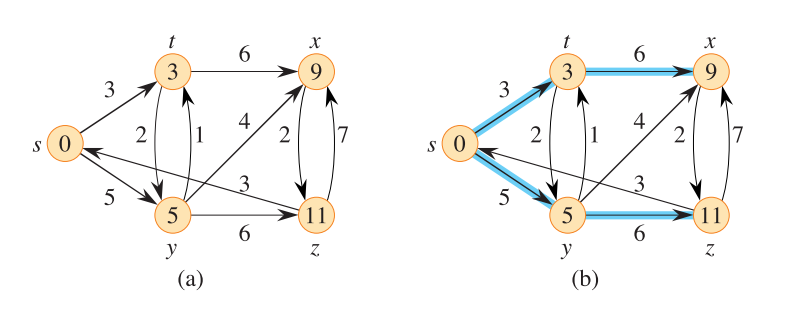
\includegraphics[scale=0.5]{shortest_path_tree.png}
\caption{(a) A weighted, directed graph with source $s$. (b) The blue edges represent the shortest-path tree rooted at the source $s$. The figure was taken from \textit{Introduction to Algorithms} by CLRS\cite{CLRS}.} 
\label{shortest_path_tree}
\end{figure}

Dijkstra algorithm is a type of greedy algorithm where it makes a locally optimal decision in each step. The following describe the high-level idea:

\begin{enumerate}
    \item At first, the source vertex only knows the distance to its neighbors and treats other vertices as if they are infinitely far away. 
    \item Among the univisited vertices, visit the vertex that is closest to the source vertex. That is, add the selected vertex to the shortest path tree and mark visited.
    \item Then, updates the distance to the vertices that are now reachable (but still unvisited) by the newly visited vertex. 
    \item Repeats the step 2-3 until all the vertex get marked visited.
\end{enumerate}


\subsection{Implementation}
In practice, the algorithm keeps track of the vertex that is closest to the source vertex using a min-priority queue. Also, the algorithm does not explicitly construct a shortest-path tree using some form of tree data structure. Rather, it records the parent pointer for each vertex. Then, the shortest path from the destination vertex to the source vertex can be found by following the parent pointers.
\autoref{dijkstra}

\begin{figure}
\centering
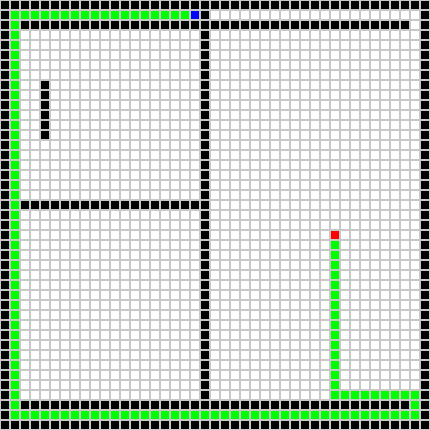
\includegraphics[scale=0.4]{dijkstra.png}
\caption{The source s is the leftmost vertex. The shortest-path estimates appear within the vertices, and blue edges indicate predecessor values. Blue vertices belong to the vertices that are marked visited, and tan vertices are the not yet visited vertices. The figure was taken from \textit{Introduction to Algorithms} by CLRS\cite{CLRS}.}
\label{dijkstra}
\end{figure}

\subsection{Pseudocode}
The following pseudocode was adapted from \textit{Introduction to Algorithms} by CLRS\cite{CLRS}.

\begin{codebox}
\Procname{$\proc{Initialize-Single-Source}(G,s)$}
\li \Comment $v.d = $ distance from $s$ to $v$
\li \Comment $v.\pi = $ parent vertex of $v$
\li
\li \For each vertex $v \in G.V$
\li     \Do
            $v.d = \infty$
\li         $v.\pi =$ NIL
        \End
\li $s.d = 0$
\end{codebox}

\begin{codebox}
\Procname{$\proc{Dijkstra}(G,w,s)$}
\li \Comment $G = (V,E);$ graph with positive weight edges
\li \Comment $s \in V$, source vertex
\li \Comment $w(u,v) = $ weight of edge $(u,v)$
\li
\li $\textsc{Initialize-Single-Source}(G,s)$
\li $S = \emptyset$ \hspace{0.5cm}\Comment Set of vertices that shortest path from $s$ is known  
\li $Q = \emptyset$ \hspace{0.5cm}\Comment Min-priority Queue
\li                 \hspace{1.5cm}\Comment Q holds unvisited vertices.
\li \For each vertex $u \in G.V$
\li     \Do
            $\textsc{Insert}(Q,u)$
        \End
\li \While $Q \neq \emptyset$
\li     \Do
            $u = \textsc{Extract-Min}(Q)$
\li         $S = S \cup \{u\}$
\li     \For each vertex $v$ in $G.Adj[u]$
\li         \Do
                \Comment found shorter way to reach $v$
\li             \If $v.d > u.d + w(u,v)$
\li                 \Do
                        $v.d = u.d + w(u,v)$    \hspace{0.5cm}\Comment Update distance to reach from $s$ to $v$
\li                     $v.\pi = u$             \hspace{2.2cm}\Comment Update parent pointer
\li                     $\textsc{Decrease-Key}(Q,v,v.d)$
                    \End
            \End
        \End
\end{codebox}

\subsection{Correctness proof}
Let $S$ be the set of vertices that are visited at some point during the algorithm. We want to prove that path found by Dijkstra results in the shortest path for all $u \in S$. 

First, consider the base case where $|S| = 1$. That is the case when $S$ contains only the source $s$. Since the distance from $s$ to $s$ is 0, it is clear that the base case holds for $|S| = 1$.

For the inductive step, assume that Dijkstra finds the shortest path for all $u \in S$, where $|S| \leq k$ for some $k \leq |V|$. Let $v$ be the $k + 1$ vertex, the next closest vertex among unvisited vertex. Let $u$ be the vertex in visited set $S$ that have closest to $v$. We want to prove that $S$ maintains the shortest path tree after visiting $v$.

We prove this by contradiction. Suppose there is another shortest path to reach $v$ through some unvisited vertex $x$ to $v$. By construction, $v$ is the closest among the unvisited vertices to some visited vertex $u$. By the inductive hypothesis, we know that path from $s$ to $u$ is the shortest. Since both path($s,u$) and path($u,v$) are shortest, the path through $x$ cannot be shorter. This contradicts the assumption that there exists a shorter path to $s$ to $v$ through some unvisited vertex $x$.
In the other words, any other path to $v$ must be longer than or equal to the path($s, u$) and then path($u, v$). This concludes that the inductive step holds for any $2 \leq k \leq |V|$. 

Therefore, Dijkstra output the shortest path for all $u \in V$ by the end of the execution when $|S| = |V|$.


\section{A* algorithm}
\subsection{"Dijkstra with a twist" \cite{Buckland}}
Most often, finding a path from $s$ to some target vertex $t$ using Dijkstra is overkill. Dijkstra algorithm finds the shortest path to all vertices from $s$ when the application only needs one shortest path from $s$ to $t$. So, the following modifications on the Dijkstra algorithm can give out better performance for finding the shortest path from $s$ to $t$. 
\begin{itemize}
    \item Dijkstra algorithm blindly selects vertex with minimum distance from $s$ each step. Instead, make a clever guess in each step where the algorithm selects a vertex that is likely part of the shortest path from $s$ to $t$.\cite{Buckland, HNR}
    \item Terminate once the shortest path from $s$ to $t$ is found.
\end{itemize}
The above modification on Dijkstra is known as the A* algorithm. Given that the A* algorithm makes an appropriate guess for each step, the A* algorithm guaranteed to return shortest path between source to target vertex. Also, the A* algorithm computationally more efficient than Dijkstra since it avoids adding unrelated shortest paths to vertices other than $t$. The guessing stretegy that A* must implement is known as admissible heuristic function.

\subsection{Admissible Heuristic}
For A* to work correctly and efficiently, the A* algorithm must guess each step that
\begin{itemize}
    \item Heuristic: \\
    Minimize unnecessary exploration on finding sub-paths that are obviously not part of the optimal path\cite{HNR}, but also 
    \item Admissibility: \\
    Should not ignore the sub-path that can be part of the optimal path\cite{HNR}. 
\end{itemize}
In many situations, there is extra information available for the given problem domain other than the distance between two vertices. For example, imagine finding the shortest route between two cities in the road network. Not only do we know the distance between two pairs of cities, but also know how all cities are positioned on the map. From this, we would unlikely consider traveling to a city in the opposite direction of a destination even if it is located close to the source. Rather, we would consider a nearby city closer to the destination unless it is deadend. 

In the above example, we considered the euclidian distance between a city and the destination in addition to the distance to reach the city. Knowing the euclidian distance was a heuristic to make an appropriate guess. That is, the goal was to select a city with minimum cost $f(v) = g(v) + h(v)$, where $g(v)$ is the exact distance to reach some city $v$ and $h(v)$ is the euclidian distance between city $v$ to destination. On the other hand, we must be sure that no overestimations were made. If we accidentally overestimate one of the sub-path that is part of the optimal path, then the optimal sub-path can be ignored due to its high cost and other non-optimal paths might be selected instead. Fortunately, the guess was safe from overestimation since it is certain that the road route cannot be shorter than the euclidian distance between them\cite{HNR}. From this, we find that euclidian distance also satisfies admissibility.


\subsection{Implementation}
Implementation is similar to Dijkstra, but the difference is that the Min-priority queue is sorted based on the cost $f$ instead of distance. Note that if no heuristic is used, $h(v) = 0$ for all $v \in V$, A* implementation is equivalent to Dijkstra.

\subsection{Pseudocode}
\begin{codebox}
\Procname{$\proc{Initialize-Single-Source}(G,s)$}
\li \Comment $v.f = $ cost of $v$: $f = g + h$
\li \Comment $v.g = $ exact distance from $s$ to $v$
\li \Comment $v.\pi = $ parent vertex of $v$
\li \Comment $h(v) = $ estimate distance from $v$ to target
\li
\li \For each vertex $v \in G.V$
\li     \Do
            $v.g = \infty$
\li         $v.f = \infty$ 
\li         $v.\pi =$ NIL
        \End
\li $s.g = 0$
\li $s.f = h(s)$
\end{codebox}

\begin{codebox}
\Procname{$\proc{A*-search}(G,s,t,w,h)$}
\li \Comment $G = (V,E);$ graph with positive weight edges
\li \Comment $s \in V$, source vertex
\li \Comment $t \in V$, target vertex
\li \Comment $w(u,v) = $ weight of edge $(u,v)$
\li \Comment $h(v) = $ estimate distance from $v$ to $t$  
\li
\li $\textsc{Initialize-Single-Source}(G,s)$
\li $S = \emptyset$ \hspace{0.5cm}\Comment Set of vertices that shortest path from $s$ is known  
\li $Q = \emptyset$ \hspace{0.5cm}\Comment Min-priority Queue sorted by cost $f$.
\li                 \hspace{1.5cm}\Comment Q holds unvisited vertices.
\li \For each vertex $u \in G.V$
\li     \Do
            $\textsc{Insert}(Q,u)$
        \End
\li \While $Q \neq \emptyset$
\li     \Do
            $u = \textsc{Extract-Min}(Q)$
\li         $S = S \cup \{u\}$
\li     \If $u = t$
\li         \Do 
                break 
\li         \End
\li     \For each vertex $v$ in $G.Adj[u]$
\li         \Do
                \Comment found shorter way to reach $v$
\li             \If $v.g > u.g + w(u,v)$
\li                 \Do
                        $v.g = u.g + w(u,v)$    \hspace{0.5cm}\Comment Update exact                    distance to reach from $s$ to $v$
\li                     $v.f = v.g + h(v)$      \hspace{0.9cm}\Comment Update cost to                                               of $v$ 
\li                     $v.\pi = u$             \hspace{2.2cm}\Comment Update parent pointer
\li                     $\textsc{Decrease-Key}(Q,v,v.f)$
                    \End
            \End
        \End
\li
\li \Return $\textsc{Path}(G,s,t)$
\end{codebox}


\section{Hierarchical Path Finding}
\subsection{Path finding algorithm for modern applications}
In practice, a naive A* algorithm is still not sufficient for many modern applications. First, many modern applications require computation to happen in real-time for hundreds, if not thousands, users/agents simultaneously\cite{Botea2004NearOH}. Secondly, the shift to mobile applications has put more limitations on memory and CPU usage\cite{Botea2004NearOH}.
For this reason, many variants of the A* algorithm such as IDA*, D*, etc have been proposed to combat the complexity of modern applications. Like many problems in computer science, one approach is to divide and conquer. That is, instead of running the A* algorithm in the whole graph, restructure the problem in a way to use the A* algorithm in a smaller sub-graph and then combine the result to find the shortest path from source to destination in an original graph. This is known as the Hierarchical Path Finding algorithm.

\subsection{Hierarchy}
Section 3.2 give an illustration of how A* mimics the decision-making process of human by use of admissible heuristic. However, A* lack the arguably most important skill that human use: abstraction. Consider the following example of how a human might plan his/her trip from Virginia Tech to the University of Virginia. The example is adapted from \textit{Near Optimal Hierarchical Path-Finding} \cite{Botea2004NearOH}.
\begin{enumerate}
    \item Plan a route from Virginia Tech to a major highway entrance in Blacksburg.
    \item Plan a route from Blacksburg to Charlottesville.
    \item Plan a route from the highway exit in Charlottesville to the University of Virginia.
\end{enumerate}
In the above example, the complexity of finding a path from Virginia Tech to the University of Virginia was reduced in each step. The traveler only needs detailed maps for two cites \cite{Botea2004NearOH}, Blacksburg and Charlottesville. Once the traveler enters the highway, a simplified highway map can be used and ignore all other road details of other cities that pass by \cite{Botea2004NearOH}.

Likewise, the idea of Hierarchical Path Finding is to form a region by clustering the vertices and introducing high-level regional routes \autoref{hierarchy}. Then, the steps for finding a path from the source vertex to the destination vertex are (1) compute a local (low-level) route to the source vertex to the source region entrance, (2) compute a regional (high-level) route from the source region to destination region, and (3) compute a local (low-level) route to destination region exit to destination vertex.

\begin{figure} 
\centering
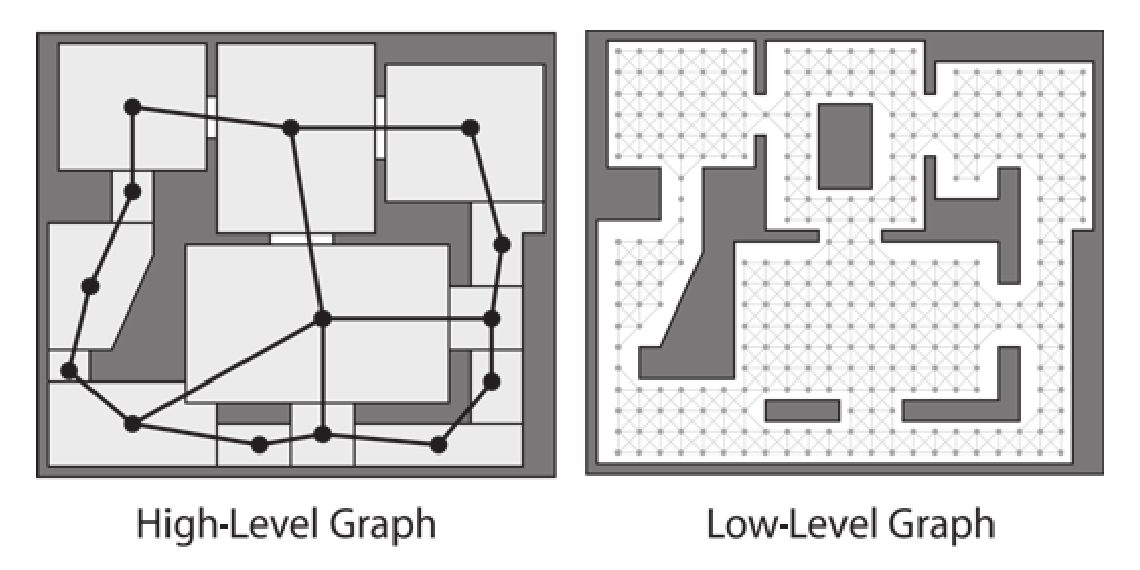
\includegraphics[scale=0.4]{hierarchy.png}
\caption{Forming regions (high-level graph) by clustering neighboring vertices. The figure was taken from \textit{Programming Game AI by Example} by Buckland\cite{Buckland}.} 
\label{hierarchy}
\end{figure}


\subsection{Time optimization: All-pair shortest path}
For applications where computational time is more critical than memory usage, caching technique can be used\cite{Buckland}. That is, the shortest path between regions can be pre-computed for all regions and stored inside a table/matrix. The simplest form is to run Dijkstra on each region, but more sophisticated algorithms should be used in practice. This is also known as finding an all-pair shortest path. Once stored inside a table/matrix, finding a regional route from the source region to the destination region can be performed in constant time during runtime. 


\subsection{Near optimal path}
One caveat of the Hierarchical Path Finding algorithm is that it does not guarantee the shortest path between the source and destination vertex. Using the human traveler analogy from section 4.2, a highway route may make travelers travel around the city, adding more distance needed to travel compared to traveling through city roads\cite{Botea2004NearOH}. The \textit{Near Optimal Hierarchical Path-Finding} apply a path-smoothing procedure to make a path found by Hierarchical Path Finding within $1\%$ optimal compared to shortest path\cite{Botea2004NearOH}.

\subsection{Implementation}
Compare to Dijkstra and naive A*, there are more tunable variables that implementers need to consider; the number of hierarchy levels, cluster/region size, and placement of regional entrances/exits. In practice, optimizations like preprocessing/caching regional routes and path smoothing may be necessary.
To avoid overwhelming the algorithm with optimization details, our implementation assumes the following simplifications: (1) an input graph is static and known in advance, (2) 2 levels of the hierarchy, (3) preselecting regional entrances/exits in reachable locations, (4) no preprocessing/caching, and (5) no path refinement or smoothing.


\subsection{Pseudocode}
\begin{codebox}
\Procname{$\proc{Hierarchical-Path-Finding}(G, s, t, w, h)$}
\li \Comment $G = (V,E);$ graph with positive weight edges
\li \Comment $s \in V$, source vertex
\li \Comment $t \in V$, target vertex
\li \Comment $w(u,v) = $ weight of edge $(u,v)$
\li \Comment $h(v) = $ estimate distance from $v$ to $t$  
\li
\li $Path = \{\}$   \hspace{3cm}\Comment Hold global path from $s$ to $t$
\li $L_2$ = $\{\}$  \hspace{3.4cm}\Comment Hold regional level path from $s$ to $t$ 
\li $G_2 = \textsc{CreateLevel2}(G)$ \hspace{0.7cm}\Comment Create regional vertices from $G$
\li $G_2.V = G_2.V \cup \{s, t\}$   \hspace{1.4cm}\Comment Add $s$ and $t$ to regional vertices
\li
\li $L_2 = \textsc{A*-search}(G_2,s,t,w,h)$     \hspace{0.5cm}\Comment Compute regional shortest path
\li
\li \Comment Compute local shortest path between two regions inside regional shortest path
\li \Comment then add to global path
\li \For $i = 1$ to $|L_2| - 1$
\li     \Do
            $L_1 = \textsc{A*-search}(G,L_2[i],L_2[i+1],w,h)$ \hspace{0.5cm}\Comment shortest path between $L_2[i]$ and $L_2[i+1]$
\li         $Path = Path \cup L_1$
        \End
\li 
\li \Return $Path$
\end{codebox}


\section{Conclusion}
The Dijkstra and A* have their strong points and cannot argue that one is better than the other in all situations. However, knowing that most applicants do not need additional computation for finding a path to all vertices from the source, A* became a preferred method of the path-finding algorithm in most cases. Hierarchical Path Finding follows the similar footstep. Many applications nowadays are more constrained by the resource than optimality, allowing Hierarchical Path Finding to rise despite its additional complexity and non-optimality. For our next step, we plan to implement and showcase the three algorithms, Dijkstra, A*, and Hierarchical Path Finding discussed in this paper. Throughout the process, we will explore whether the performance of Hierarchical Path Finding is worth the additional complexity.


\medskip
 
\bibliographystyle{plain}
\bibliography{references}
 
\end{document}